\begin{figure*}[t]
    \centering
    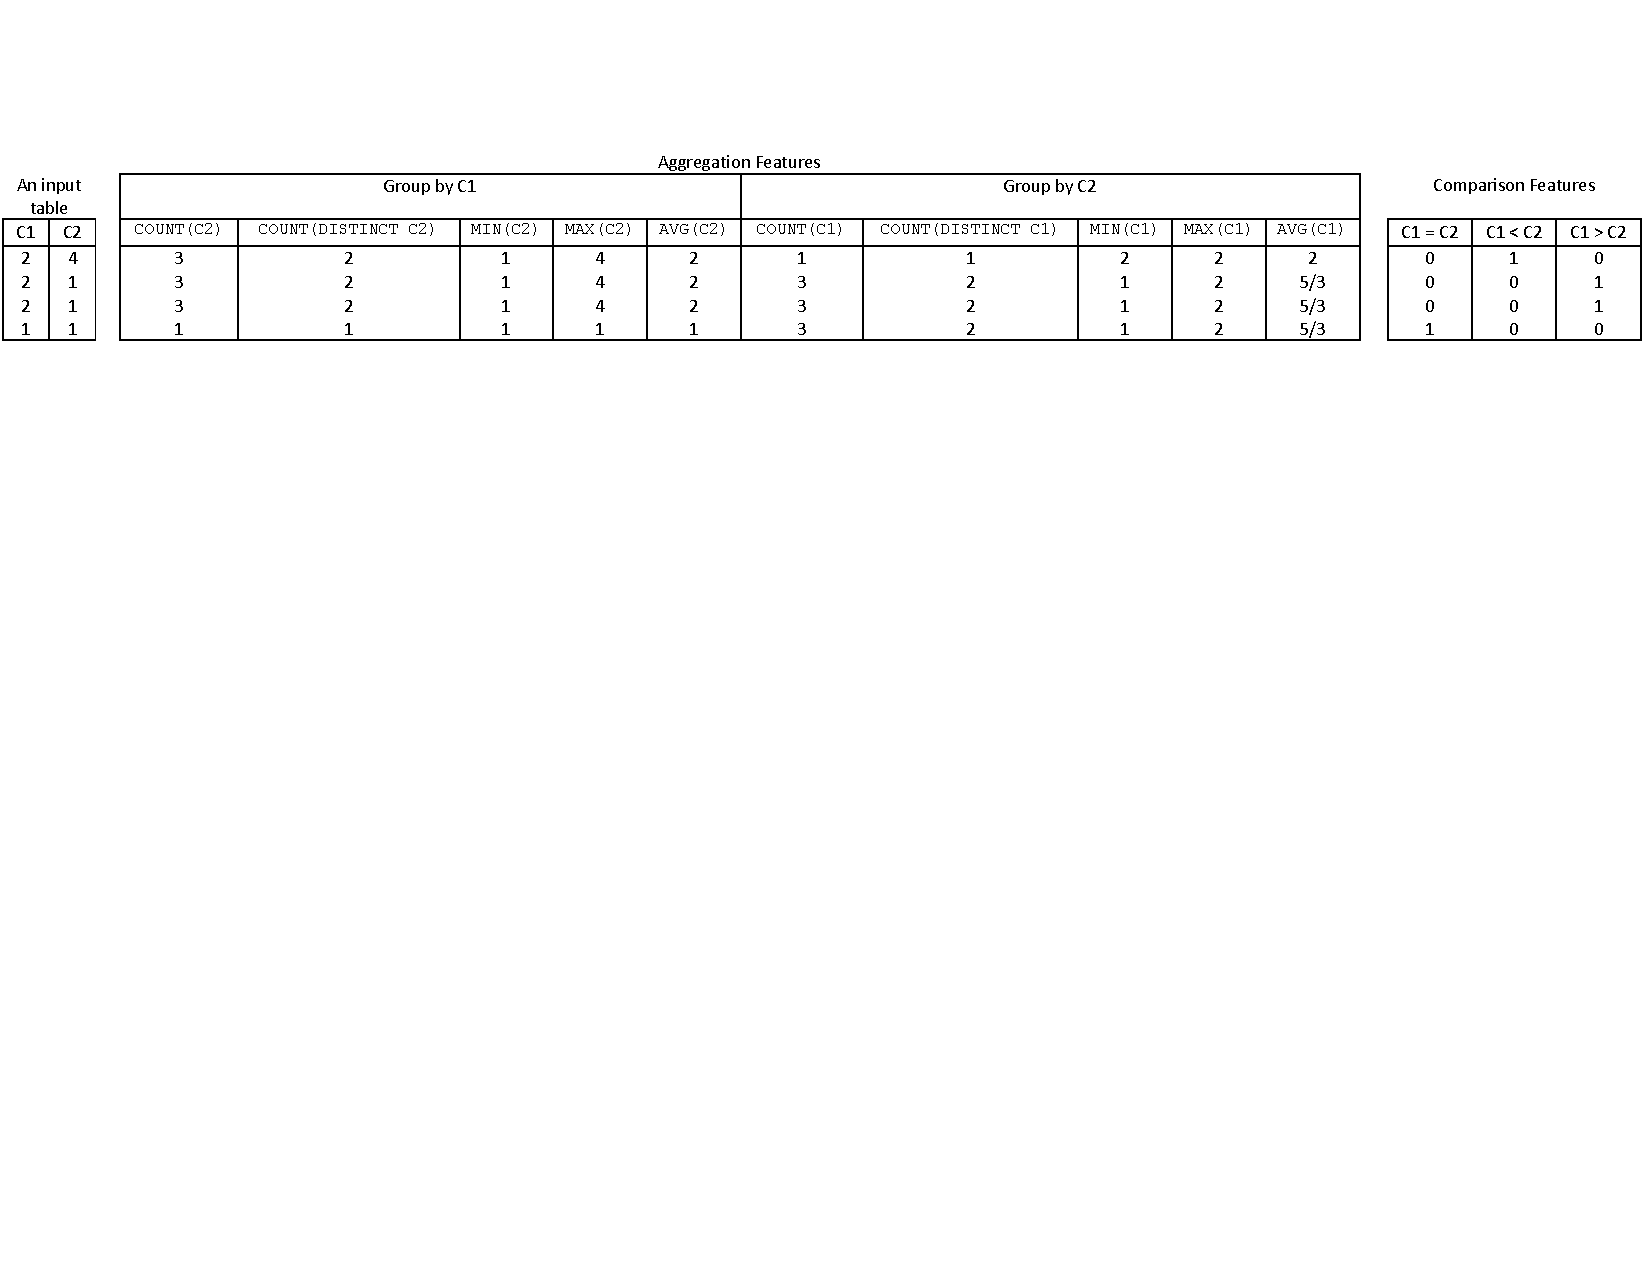
\includegraphics[scale=0.66]{featurex}
    \vspace{-7mm}
	\caption{Illustration of two types of additional features
    added by \ourtool. (Left) An example input table with
    two columns: C1 and C2. (Center) The aggregation features added by
    \ourtool for the input table. (Right) The comparison features
    added by \ourtool for the input table.
    Take the first cell in the input table as an example,
    when grouping the table by column C1 (with value 2), the count
    of values in the C2 column is 3; the count of
    distinct values in the C2 column is 2; the minimal value
    in the C2 column is 1, the maximal value in the C2 column
    is 4, the sum of values in the C2 column is 6,
    and the average value of the C2 column is 2.
   % Similar results can be computed if the table is grouped by the C2 column.
}
	\label{fig:features}
\end{figure*}
